%%%%%%%%%%%%%%%%%%%%%%%%%%%%%%%%%%%%%%%%%%%%%%%%%%%%%%%%%%%%%%%%%%%%%%%%%%%%%%%%
% > Лабораторная работа 7: Поперечные колебания круглой пластины.
% > Баталов Семен, Антонова Мария, Клюшин Максим, Хайретдинова Диана.
% > 2021 год.
%%%%%%%%%%%%%%%%%%%%%%%%%%%%%%%%%%%%%%%%%%%%%%%%%%%%%%%%%%%%%%%%%%%%%%%%%%%%%%%%

\documentclass[12pt, a4paper]{article}
\usepackage[left=2cm, right=2cm, top=2.5cm, bottom=2.5cm, nohead, 
footskip=1cm]{geometry}
\usepackage{graphicx}
\graphicspath{{./Pictures/}}
\usepackage[utf8]{inputenc}
\usepackage[english, russian]{babel}
\usepackage{indentfirst}
\usepackage{array}
\usepackage{longtable}
\usepackage{misccorr}
\usepackage{setspace, amsmath}
\usepackage{multirow}

\begin{document}
    
    \newcolumntype{M}[1]{>{\centering\arraybackslash}m{#1}}
    \renewcommand{\arraystretch}{1.4}
    
    \begin{center}
        \large{Санкт-Петербургский государственный университет} \\
        \large{Saint-Petersburg State University}\\
        \hfill \break
        \hfill \break
        \hfill \break
        \hfill \break
        \hfill \break
        \hfill \break
        \hfill \break
        \large{Кафедра теоретической и прикладной механики} \\
        \hfill \break
        \hfill \break
        \large{\textbf{ОТЧЕТ}} \\
        \large{\textbf{По лабораторной работе 7}} \\
        \large{<<Поперечные колебания круглой пластины>>} \\
        \hfill \break
        \hfill \break
        \hfill \break
        \large{По дисциплине} \\
        \large{<<Лабораторный практикум по теоретической механике>>} \\
    \end{center}
    
    \hfill \break
    \hfill \break
    \hfill \break
    \hfill \break
    \hfill \break
    \hfill \break
    
    \begin{flushright} 
        \large{Выполнили:} \\
        \hfill \break
        \large{Баталов С. А.} \\
        \large{Антонова М. Н.} \\
        \large{Клюшин М. А.} \\
        \large{Хайретдинова Д. Д.} \\
    \end{flushright}
    
    \hfill \break
    \hfill \break
    \hfill \break
    \hfill \break
    
    \begin{center} 
        \large{Санкт-Петербург} \\
        \large{2021} \\
    \end{center}
    
    \thispagestyle{empty}
    \newpage
    \sloppy
    
    \section{Описание установки}
    
    В этой лабораторной работе анализируются поперечные колебания круглой упругой пластины. Целью работы является экспериментальное определение собственных частот поперечых колебаний упругой пластины, наблюдение соответствующих собственных форм колебаний и сравнение экспериментально определенных собственных частот с их расчетными значениями. В процессе исследовая формы колебаний определяются с помощью фигур Хладни.
    
    \begin{figure} [h]
        \centering
        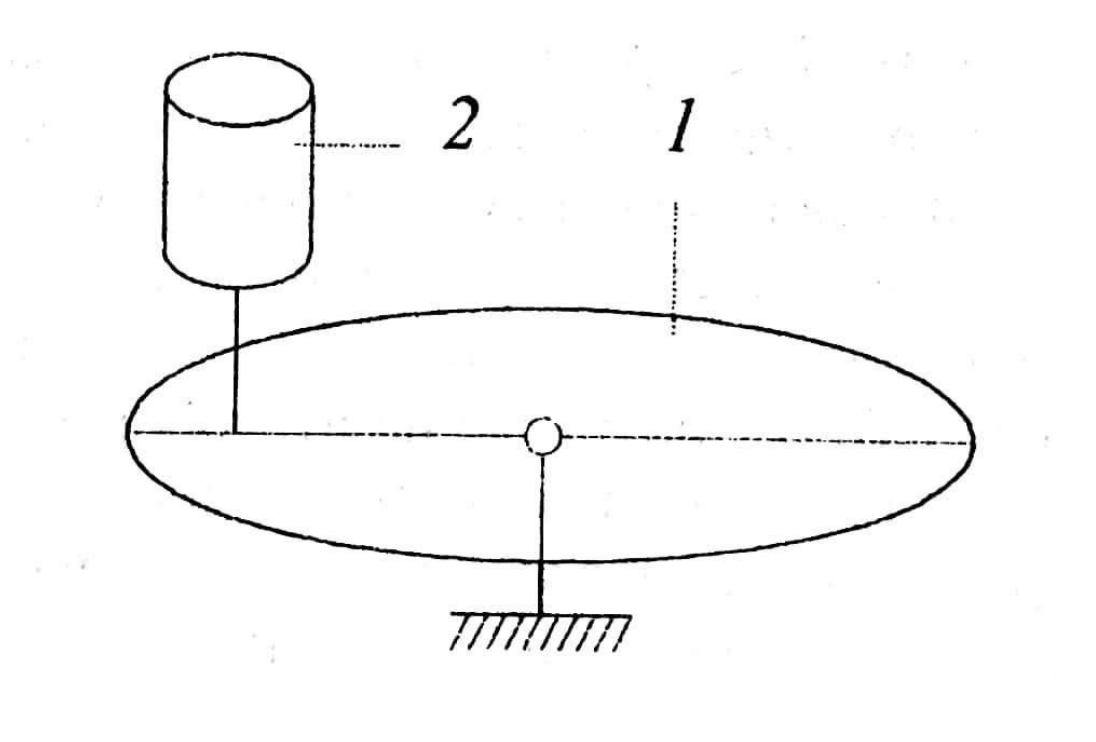
\includegraphics [width = 13cm] {Lab_7_1.png}
        \caption{\centering Схема лабораторной установки.}
        \label{im1}
    \end{figure}
    
    3кспериментальная установка, показанная на рис.~\ref{im1}, представляет собой круглую упругую пластину \textit{1}, жестко закрепленную по краям центрального отверстия и свободную на внешнем крае. К пластине присоединена тяга электромагнита \textit{2}, питаемого переменным током звуковой частоты от генератора. Электромагнит предназначен для создания периодической возмущающей силы, прикладываемой к пластине, частота возмущающей силы равна частоте переменного тока.
    
    \newpage
    
    \section{Параметры установки}
    
    В следующей таблице представлены заранее известные параметры установки: плотность материала пластины~--~$\rho$, коэффициент Пуассона~--~$\sigma$, модуль упругости~--~$E$, толщина пластины~--~$h$, внешний радиус пластины~--~$R$, диаметр внутреннего отверстия~--~$d$.
    
    \begin{longtable}{| M{2cm} | M{3cm} | M{3cm} | M{3cm} |}
        \caption{\centering Известные параметры.}
        \label{tb1} \\
        \hline
        Номер & Величина & Значение & Размерность \\
        \hline
        1 & $\rho$ & 2850 & $\text{кг} / \text{м}^{3}$ \\
        2 & $\sigma$ & 0,5 & -- \\
        3 & $E$ & $7 \cdot 10^{10}$ & Па \\
        \hline
        4 & $h$ & 0,003 & м \\
        5 & $R$ & 0,240 & м \\
        6 & $d$ & 0,008 & м \\
        \hline
    \end{longtable}
    
    \newpage
    
    \section{Результаты экспериментов}
    
    Далее представлены главные формы и соответствующие им частоты собственных колебаний пластины, которые были получены в ходе эксперимента.
    
    
\end{document}